% Tabellen und Vektorgrafik ausschließlich für die Lesefassung.
\definecolor{franklblue}{RGB}{34,92,133}
\definecolor{franklshade}{RGB}{226,237,244}

\newcommand{\FranklIncidenceTable}{%
  \par\medskip\noindent
  \begin{minipage}{\linewidth}
    \centering\small
    \textbf{Fünf Mengen, drei Vorkommenszahlen}\par\medskip
    \begingroup
    \setlength{\tabcolsep}{14pt}
    \renewcommand{\arraystretch}{1.25}
    \begin{tabular}{lccc}
      \toprule
      Menge \(X\in M\) & \(a\in X\) & \(b\in X\) & \(c\in X\)\\
      \midrule
      \(\varnothing\) & 0 & 0 & 0\\
      \(\{a,b\}\) & 1 & 1 & 0\\
      \(\{a,c\}\) & 1 & 0 & 1\\
      \(\{b,c\}\) & 0 & 1 & 1\\
      \(\{a,b,c\}\) & 1 & 1 & 1\\
      \midrule
      Vorkommenszahl & 3 & 3 & 3\\
      \bottomrule
    \end{tabular}
    \endgroup
    \par\medskip\raggedright
    Eine Eins bedeutet: Das Element liegt in der Menge dieser Zeile.
    Jede Spaltensumme zählt die Mengen, in denen das betreffende
    Element vorkommt. Alle drei Summen sind größer als \(5/2\).
  \end{minipage}\par\medskip
}

\newcommand{\FranklFourClassTable}{%
  \par\medskip\noindent
  \begin{minipage}{\linewidth}
    \centering\small
    \textbf{Die vier Klassen im Leitbeispiel}\par\medskip
    \begingroup
    \setlength{\tabcolsep}{11pt}
    \renewcommand{\arraystretch}{1.6}
    \begin{tabular}{c|cc}
       & \(b\notin X\) & \(b\in X\)\\\hline
      \(a\notin X\) & \(M_{00}=\{\varnothing\}\)
                   & \(M_{01}=\{\{b,c\}\}\)\\
      \(a\in X\) & \(M_{10}=\{\{a,c\}\}\)
                 & \(M_{11}=\{\{a,b\},\{a,b,c\}\}\)
    \end{tabular}
    \endgroup
    \par\medskip\raggedright
    Die Indizes geben zuerst das Auftreten von \(a\), dann das von
    \(b\) an. Die Einträge zeigen die Teilfamilien im Leitbeispiel.
    Obere und untere Zeile trennen nach \(a\), linke und rechte
    Spalte nach \(b\).
  \end{minipage}\par\medskip
}

\newcommand{\FranklRareTripleTable}{%
  \par\medskip\noindent
  \begin{minipage}{\linewidth}
    \centering\small
    \textbf{19 Mengen: \(a,b,c\) kommen jeweils nur neunmal vor}\par\medskip
    \begingroup
    \setlength{\tabcolsep}{9pt}
    \renewcommand{\arraystretch}{1.13}
    \begin{tabular}{l|ccc|cccc}
      \toprule
      Menge \(X\in M\) & \(a\) & \(b\) & \(c\)
                       & \(d\) & \(e\) & \(f\) & \(g\)\\
      \midrule
      \(\varnothing\) & 0 & 0 & 0 & 0 & 0 & 0 & 0\\
      \(A\)            & 1 & 1 & 1 & 0 & 0 & 0 & 0\\
      \midrule
      \(D_a\)                & 0 & 0 & 0 & 1 & 1 & 0 & 1\\
      \(D_a\cup\{a\}\)       & 1 & 0 & 0 & 1 & 1 & 0 & 1\\
      \(D_a\cup A\)          & 1 & 1 & 1 & 1 & 1 & 0 & 1\\
      \midrule
      \(D_b\)                & 0 & 0 & 0 & 1 & 0 & 1 & 1\\
      \(D_b\cup\{b\}\)       & 0 & 1 & 0 & 1 & 0 & 1 & 1\\
      \(D_b\cup A\)          & 1 & 1 & 1 & 1 & 0 & 1 & 1\\
      \midrule
      \(D_c\)                & 0 & 0 & 0 & 0 & 1 & 1 & 1\\
      \(D_c\cup\{c\}\)       & 0 & 0 & 1 & 0 & 1 & 1 & 1\\
      \(D_c\cup A\)          & 1 & 1 & 1 & 0 & 1 & 1 & 1\\
      \midrule
      \(B\)                  & 0 & 0 & 0 & 1 & 1 & 1 & 1\\
      \(B\cup\{a\}\)         & 1 & 0 & 0 & 1 & 1 & 1 & 1\\
      \(B\cup\{b\}\)         & 0 & 1 & 0 & 1 & 1 & 1 & 1\\
      \(B\cup\{c\}\)         & 0 & 0 & 1 & 1 & 1 & 1 & 1\\
      \(B\cup\{a,b\}\)       & 1 & 1 & 0 & 1 & 1 & 1 & 1\\
      \(B\cup\{a,c\}\)       & 1 & 0 & 1 & 1 & 1 & 1 & 1\\
      \(B\cup\{b,c\}\)       & 0 & 1 & 1 & 1 & 1 & 1 & 1\\
      \(B\cup A\)            & 1 & 1 & 1 & 1 & 1 & 1 & 1\\
      \midrule
      Vorkommenszahl & 9 & 9 & 9 & 14 & 14 & 14 & 17\\
      \bottomrule
    \end{tabular}
    \endgroup
    \par\medskip\raggedright
    Eine Eins bedeutet Mitgliedschaft, eine Null Abwesenheit.
    Die waagerechten Linien trennen die Bausteine der Familie.
    Links stehen die drei Elemente von \(A\), rechts die vier von
    \(B\). Jede Zeile ist verschieden; die Spaltensummen zählen
    die Vorkommen.
  \end{minipage}\par\medskip
}

\newcommand{\FranklInjectionDiagram}{%
  \par\medskip\noindent
  \begin{minipage}{\linewidth}
    \centering
    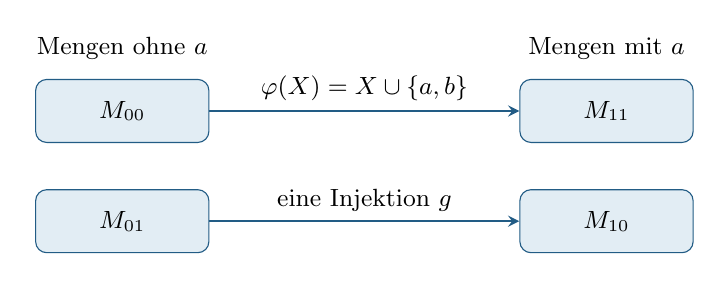
\begin{tikzpicture}[x=1cm,y=1cm,font=\small,>=stealth,
      family/.style={draw=franklblue,fill=franklshade,rounded corners,
        minimum width=2.2cm,minimum height=.8cm,inner sep=5pt}]
      \node at (0,2.05) {Mengen ohne \(a\)};
      \node at (6.15,2.05) {Mengen mit \(a\)};
      \node[family] (zero) at (0,1.25) {\(M_{00}\)};
      \node[family] (full) at (6.15,1.25) {\(M_{11}\)};
      \node[family] (mixedb) at (0,-.15) {\(M_{01}\)};
      \node[family] (mixeda) at (6.15,-.15) {\(M_{10}\)};
      \draw[->,thick,franklblue] (zero) -- node[above,text=black]
        {\(\varphi(X)=X\cup\{a,b\}\)} (full);
      \draw[->,thick,franklblue] (mixedb) -- node[above,text=black]
        {eine Injektion \(g\)} (mixeda);
    \end{tikzpicture}
    \par\medskip\small\raggedright
    Dieser Fall gilt bei \(|M_{01}|\leq|M_{10}|\).
    Jeder Pfeil ist injektiv. Ihre Zielklassen sind disjunkt:
    Oben enthalten alle Mengen \(b\), unten enthält keine \(b\).
    Daher sind auch Bilder verschiedener Zweige stets verschieden.
  \end{minipage}\par\medskip
}
